%!TEX root = Slic3r-Manual.tex

\subsection{Understanding extrusion width}
\label{sec:understanding_extrusion_width}
\index{Extrusion Width}
\index{Flow Math}
\index{Extrusion Overlap}

Two main questions affect Slic3r's work:
\begin{itemize}
\item How distant should extrusion paths be positioned in order to get a good continuous finish?
\item How much material must be extruded along such paths?
\end{itemize}

If two adjacent paths are too close (or too much material is extruded), they'll overlap. If two adjacent paths are too distant (or not enough material is extruded), gaps will be visible and/or the extrusions will delaminate because of not enough bonding.

By extruding more or less while moving (i.e. by changing the flow speed/head speed ratio) we can make paths thicker or thinner:

\begin{figure}[H]
\centering
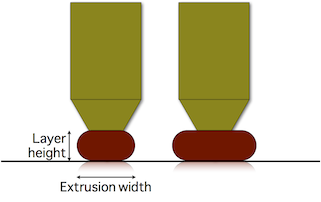
\includegraphics[keepaspectratio=true,width=.66\textwidth]{advanced/flow_math/extrusion-width.png}
\caption{Extrusion Width.}
\label{fig:extrusion-width}
\end{figure}

Thicker paths will have better bonding with the lower layer, thus are good for mechanical parts. However, they'll be less able to approximate the object shape and fill tiny gaps or narrow curves (think of a drill bit: a larger one will not be able to enter narrow places). On the contrary, thinner paths will provide less bonding but better shape accuracy.

However note that extrusion width can be controlled only when extruding over an existing surface (such as a previous layer or print bed). If we extrude in free air (i.e. when bridging), the resulting shape will be always round and equal to the nozzle diameter:

\begin{figure}[H]
\centering

\includegraphics[keepaspectratio=true,width=.5\textwidth]{advanced/flow_math/bridge.png}
\caption{Bridging filament shape.}
\label{fig:bridge}
\end{figure}

If you reduce the material flow you'll get smaller circles to some extent, until the plastic viscosity decides it's time to break your bridge because of too much tension. If, on the contrary, you extrude too much material, the shape of the extruded filament won't change (still equal to nozzle diameter) but you'll get a loose bridge.

Let's start from a definition:

\begin{description}
\item[Extrusion Width] is the thickness of a single filament extruded either in free air or above a surface. It's not the distance of two adjacent paths since some overlap will be generally applied in order to get better bonding.
\end{description}

\subsection{Bridges: the easy case}
\label{sec:bridges}
\index{Bridging}
\index{Bridge}

As said above, there's only one correct flow rate for bridging: the one that doesn't make your bridge sag or break. Extrusions are round and their diameter is equal to the nozzle diameter. Parallel paths will be positioned so that they are tangent, thus the spacing between one path and its neighbor is equal to nozzle diameter as well. (In case of bridges, we want no overlap because it has proven to drag the existing paths.)

The required material volume for a path of unitary length is calculated accordingly to the cylindric shape, thus with a circular cross-sectional area:

\verb|E = (nozzle_diameter/2)\textasciicircum{2} * Pi|

\subsection{Extruding on top of a surface}
\label{sec:extruding_on_surface}
\index{Extrusion Shape}
\index{Extrusion Width}

In this case the problem is: what shape will our extrusion get? We know it will get squashed horizontally, but will it have a rectangular or oval shape? What's the maximum extrusion width we can get with a given nozzle diameter before plastic starts curling at the sides?

Slic3r assumes that the cross-sectional shape of an extrusion is a rectangle with semicircular ends. So the relationship between desired extrusion width and volume to extrude is the following:

\begin{figure}[H]
\centering
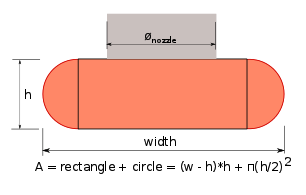
\includegraphics[keepaspectratio=true,width=.66\textwidth]{advanced/flow_math/area1.png}
\caption{Extrusion shape.}
\label{fig:area1}
\end{figure}

When target extrusion width is thinner than layer height the shape is unpredictable so we just use the same rectangular formula but discourage usage of such thin extrusion values.

The above formula provides a function that correlates the target extrusion width with the amount of material to extrude per distance unit:

\par \verb|E = f(extrusion width layer_height)|

\subsection{Spacing paths}
\label{sec:spacing_paths}
\index{Paths}

How much should we overlap paths in order to get perfect bonding?
Supposing no overlap, thus tangent paths, there would be empty space (yellow):

\begin{figure}[H]
\centering
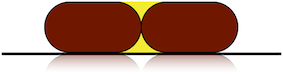
\includegraphics[keepaspectratio=true,width=.66\textwidth]{advanced/flow_math/tangent.png}
\caption{No path overlap}
\label{fig:tangent}
\end{figure}

The cross-section area of such voids is generally:

\par \verb|void area = layer height\^{2} - (layer height/2)\^{2} * PI|

Ideally, we would want to fill all of that yellow area by placing the extrusions closed to each other. However, it's very unlikely that the second extrusion will fill the space below the previous one, so there would still be a little void. The ideal overlap would be something like:
\par \verb|0 < overlap factor * void area < void area|
with overlap factor ranging from 0 to 1. Overlap factor represents how much void remains between the extrusions. It's difficult to estimate this amount, since it probably depends also on viscosity of plastic, extrusion speed and temperature. In the past, several values were tried for overlap factor, but some users were still reporting too sparse paths. A value of 1 is currently being used to guarantee that the error (which is always present) is fully on the side of abundant extrusion rather than lacking material.

Path spacing is thus:
\par \verb|spacing = extrusion width - layer height * (1 - PI/4)|

\subsection{Sane defaults}
\label{sec:sane_defaults}
\index{Sane Defaults}

Slic3r allows users to define extrusion width manually for each kind of extrusion (perimeters, infill, support material etc.) but will calculate sane defaults if no custom values are entered.
For the outermost loop of perimeters (aka external perimeters) Slic3r will default to a thin extrusion width, equal to 
\par \verb| nozzle diameter * 1.05|.

This is considered the thinnest safe extrusion width. A thin extrusion width provides better accuracy to the object shape and minimizes the flow errors caused by irregular filament.

Extrusion width for other things is calculated by getting the cross-sectional area of the configured nozzle diameter and then calculating the extrusion width produced by extruding that amount of material. In other words, by matching flow speed and head speed. The purpose of this logic is to find the "native" flow that minimizes side forces during extrusion. Such calculated extrusion with is capped to max value equal to:
\verb| nozzle diameter * 1.7|, except for internal sparse infill where the full native flow is used.
